\chapter{Introduction}
\section{But why}
\section{Requirement engineering}
% Written by Andreas
In a complex system, there are many stakeholders, both internal and external.
The requirements are meant to capture the needs of the users and convey them to
the developers \cite{ibm_req}. It is important that the requirements are
unambiguous \cite{ibm_req, rupp2014}. Since natural language is ambiguous by
nature, there are framewortks and templates to improve the quality of the
requirements \cite{rupp2014}. 

\subsection{User and system requirements}
Requirements can be organized into two categories, User and System requirements.
These differ in a number of ways, both in their nature and how they are
procured.

A project design starts with a need from a customer or user. These needs set the
goal of the project and are of a high level, abstract nature. They are captured
from the future users of the system and are expressed in the users language. In
essence, the User requirements describe the problem that is to be solved by the
system \cite{ibm_req}. 

When the User requirements are set, they need to be condensed into technical
requirements that the developers can work towards. These are the System
requirements. They define what the system and its sub-systems do. It is the
deveoplers that own these requirements and they are responsible that these in
turn fulfill the User requirements \cite{ibm_req}.

In the Eco Cars project, the stakeholders and the developers are the same
entity. This means that techniques for eliciting requirements specified by IBM
\cite{ibm_req} such as interviews are not applicable. A certain disconnect
between developers and users can be beneficial to reduce the risk of mixing the
priorities of the project goals, e.g setting too lenient user requirements
because the developing limitations are known at the requirement setting stage.
%% COMMENT: I have no source on the above, it is just a personal opinion.
To set clear boundaries between user and developer in the project, user
requirements are, where possible, sourced from the Shell Eco Marathon rules.

\subsection{Requirement formulation}
It is important that requirements are clear and unambiguous. By using templates
when expressing the requirements, there is a framework where it is agreed what a
word/phrase means. This greatly increases the quality of the requirements
\cite{rupp2014}. By using a template for the structure of a requirement, it is
ensured that all parts needed are in the requirement. Rupp \cite{rupp2014}
gives a template on how to formulate a requirement \ref{fig:req_template}.

\begin{figure}[H]
    \centering
    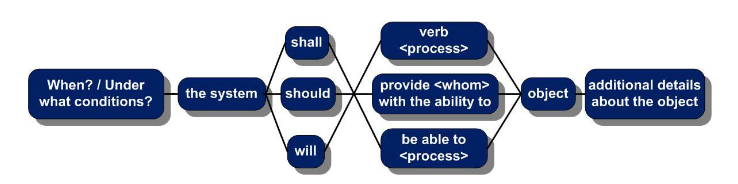
\includegraphics[width=\textwidth]{./img/introduction_req_template}
    \label{fig:req_template}
    \caption{Requirement formulation template.}
\end{figure}

To convey the relevant information, each requirement needs some metadata
connected to it. Thses metadata makes it possible to see the cicumstances under
which the requirement was set and will be tested, who is responsible and when
changes are made. These attributes allow requirements to be grouped and searched
\cite{ibm_req}.

In \cite{ibm_req}, a number of relevant metadata attributes are provided.
Together these make up a comprehensive view of each requirement. Since the Eco
Cars project is of medium size, attributes related to subsystems are not needed
since there are not many layers in the system architecture. In the project, the
requirement attributes that are used are displayed in Table~\ref{tab:req_attr}.

\begin{figure}[H]
    \centering
    \label{tab:req_attr}
    \caption{Requirement attributes used in the Eco Cars project.}
    \begin{tabular}{r | l }
        \bf{Status} & Stage in acceptation process. \\
        \hline
        \bf{Author} & Requirement author. \\
        \hline
        \bf{Created date} & Date when requirement was proposed. \\
        \hline
        \bf{Latest change by} & Last person that made changes to requirement. \\
        \hline
        \bf{Latest change date} & Date when requirement was last changed. \\
        \hline
        \bf{Dependencies} & Requirements that this depends on. \\
        \hline
        \bf{Requirement} & Natural language formulation of requirement. \\
        \hline
        \bf{Comment} & Signed comment to each change made.
    \end{tabular}
\end{figure}

\subsection{Requirement software}
In a complex system, there are many relationships between stakeholders and
requirements \cite{ibm_req}. Since requirements are the result of a process
where a large problem is divided into smaller parts, a change in one requirement
may affect several other requirements. Therefore, it is important to have a
requirement software that makes it easy to track the dependencies between the
different requirements \cite{ibm_req}. It is also important that it is easy for
the user to see, edit and create new requirements.

There are a number of Requirement Engineering programs available, such as IBM
Rational Doors, Siemens Polarion and RequisitePro. These all provide solutions
for creating, managing and tracking requirements in projects. All of these can
be used under paid licenses. Of these, only Doors is available to use for the
Eco Cars team since a license is provided by KTH. Doors is very full featured
and the group have some use experience from previous courses. 

The features required in this project are the requirement organization, inter
requirement tracking and test case linkning. These are part of the core set of
functionalities of Doors, there are many more features that can be used. The
redundancy of features clutters the UI and makes the program less easy to use.
Because of this, an alternative solution was chosen. The goal of this
requirements solution was to have a clean, easy to use UI that only implements
the features that are needed in the project, but at the same time was
extensible so that additional features could easily be added as needed.

The chosen implementation was an html document made with
Markdown(http://daringfireball.com). Markdown is a language that uses simple
syntax to create Markdown files (file extension .md) that are then parsed
into standard HTML. The HTML implementation allowed for linking of requirements,
both internally in the document but also externally to files in the project
folder structure using the HTML anchor-tag (<a>). To simplify the creation of
new requirements, a HTML/CSS/JavaScript local web page was created. This web
page allows the user to create syntactically correct requirements according to
the standard set by the team using a graphical UI. Using an automated solution
to generate requirement code reduces the risk of errors and makes the process of
creating new requirements less tedious and more intuitive. Should the
requirement standard format be changes, for example by adding an attribute, the
script can easily be updated and new requirements will follow the standard.

\subsubsection{Requirement format and Markdown}
Markdown uses a simple syntax to edit and typeset documents. The Markdown
document is parsed into HTML (sometimes with additional styling in CSS) using a
parser program. There are a variety of free parsers. A full reference to the
Markdown syntax is available on the home page of the language but the relevant
elements are given in {\bf appendix}. %% This needs to be added to an appendix
%% and referenced to this // AF
%% TODO: Continue the section detailing what the format of the requirements is
%% what they look like in markdown.

